\section{Описание решения}
В этой главе подробно рассмотрен весь алгоритм распознавания речевых команд. Для удобства понимая названия параграфов расположены в том же порядке, что и этапы в самом алгоритме.

\subsection{Предобработка}
Каждая команда - это звуковой wav файл. В каждом файле - набор амплитудных значений, которые были получены в результате записи команд дикторами. 

\subsubsection{Нормализация сигнала}
В начале проводится нормализация амплитуд. Каждое значение амплитуды приводится к такому значению, чтобы минимум среди всех амплитуд звуковой дорожки был в 0, а максимум среди всех - в 1 по формуле:
\begin{equation}
	\overline{x}_i=\dfrac{x_i}{\max_{j} |x_j|},~i=\overline{0, p-1},~j \in [0, p-1]
\end{equation}
где $x$ - значение амплитуды, $\overline{x}$ - новое значение амплитуды, $p$ - количество амплитудных значений в звуковой дорожке.

Таким образом все значения амплитуд принимают значения в диапазоне $[0,1]$.

\subsubsection{Удаление постоянной составляющей}
Постоянная составляющая (DC-offset) - это смещение амплитуды сигнала на некоторую постоянную величину. Возникает это в аналого-цифровом сигнале из-за разницы напряжения между звуковой картой и устройством ввода. Данный эффект является помехой, от которой нужно избавиться. Для этого необходимо вычесть из каждого значения амплитуды среднее арифметическое всех значений амплитуд по формуле:
\begin{equation}
\overline{x}_i=x_i - \sum_{j=0}^{p-1} x_j,~i=\overline{0, p-1}
\end{equation}
где $x$ - значение амплитуды полученное на этапе нормализации, $\overline{x}$ - новое значение амплитуды, $p$ - количество амплитудных значений в звуковой дорожке.

\subsubsection{Выделение начальной и конечной точек слова}
Каждая звуковая дорожка содержит в себе помимо фрагментов звукового сигнала - команды ещё и фрагменты тишины. Очень важно отделить звуковой сигнал от фрагментов тишины, т. к. именно он несёт в себе всю информацию о команде. 

Для того, чтобы выделить звуковой сигнал и <<обрезать>> тишину в начале и в конце записи, используется алгоритм, описанный статье \cite{SignalPreprocessing}. 
Каждая звуковая дорожка разбивается на фреймы - наборы амплитуд, каждый длительностью 20 мс. Начала фреймов расположены с периодичностью 10 мс. Таким образом, фреймы пересекаются между собой. Это обеспечивает целостность обработки звукового сигнала, т.е. позволяет не упустить важные фонемообразующие особенности.

Затем для каждого фрейма вычисляется мгновенная энергия:
\begin{equation}
E_k = \sum_{m=0}^{N-1} x_{k_m}^2,~k=\overline{0,z-1}
\end{equation}
где $z$ - количество фреймов для конкретной звуковой записи, N - длина одного фрейма (количество амплитуд в одном фрейме).

Мгновенная энергия имеет один значительный недостаток. У неё очень большая чувствительность к относительно большим значениям амплитуды из-за возведения во вторую степень. Это ведёт к искажению соотношений отсчётов звукового сигнала между друг другом. Поэтому функция мгновенной энергии переопределяется как:
\begin{equation}
\label{eq:instant_energy}
E_k = \sum_{m=0}^{N-1} |x_{k_m}|,~k=\overline{0,z-1}
\end{equation}

После того, как посчитаны мгновенные энергии для каждого фрейма, вычисляется нижнее и верхнее пороговые значения:
\begin{equation}
\begin{aligned}
& I_1 = 0.03 \cdot (MX - MN) + MN \\
& I_2 = 4 \cdot MN \\
& ITL = min(I_1,~I_2)\\
& ITU = 10 \cdot ITL
\end{aligned}
\end{equation}
где $MN$, $MX$ - минимум и максимум мгновенной энергии среди всех фреймов соответственно, $ITL$, $ITU$ - нижнее и верхнее пороговое значение.

Происходит поиск фрейма, с которого начинается слово с самого первого фрейма. Фрейм, в котором значение мгновенной энергии превышает $ITL$, предварительно помечается как начало слова. Затем начиная с этого помеченного фрейма происходит поиск фрейма, в котором значение мгновенной энергии превышает $ITU$. Если значение мгновенной энергии для какого-то фрейма во время последнего поиска меньше $ITL$, то этот фрейм становится предварительным началом слова. 

Аналогично происходит поиск конца слова в звуковой дорожке. Только поиск по фреймам происходит не с начала сигнала, а с конца.

После этого этапа имеются два предварительно помеченных фрейма $m_1, m_2$  - начало и конец слова в звуковом файле.

Функция мгновенной энергии, определённая формулой \eqref{eq:instant_energy} хорошо справляется с отделением звонких звуков от тишины. Но вот глухие она отделяет плохо. Поэтому используется вторая характеристика для доопределения начала и конца слова - число переходов через ноль. Это количество таких случаев, когда соседние отсчёты (значения амплитуд) имеют противоположные знаки. Определяется формулой:
\begin{equation}
	Z_k = \dfrac{1}{2} \sum_{m=1}^{N-1} |sgn(x_{k_{m-1}}) - sgn(x_{k_m})|,~k=\overline{0,z-1}
\end{equation}
Подразумевается, что первые 100 мс звуковой записи - это тишина, и речь начинается позднее.

Вычисляется среднее значение переходов через ноль в течение первых 100 мс \eqref{eq:izc},  среднее квадратическое отклонение количества переходов через ноль в течение первых 100 мс \eqref{eq:deviation}:
\begin{align}
	\label{eq:izc}
	&IZC = \dfrac{1}{z} \sum_{k=0}^{z-1} Z_k \\
	\label{eq:deviation}
	&\sigma_{IZC} = \sqrt{\dfrac{1}{z} \sum_{k=0}^{z-1} (Z_k - IZC)^2}
\end{align}
а затем пороговую функцию числа переходов через ноль по формуле:
\begin{equation}
	IZCT = min(IF,~IZC + 2 \sigma_{IZC}),
\end{equation}
где $IF$ - фиксированное количество переходов через ноль. В данном случае 
то 25 пересечений за 10 мс, то есть $IF=2.5$. 

Происходит уточнение точек начала и конца слова в звуковой дорожке. Начиная от фрейма $m_1$ влево происходит поиск фреймов, у которых число переходов через ноль выше порогового значения. Поиск происходит всего на расстоянии 25 фреймов, так как производится уточнение границ слова. Если пороговое значение было превышено 3 или более раз, то фрейм $r_1$, где это произошло впервые, помечается как начало слова.

Аналогично от фрейма $m_2$ происходит поиск вправо для уточнения точки конца слова.

В результате имеется 2 помеченных фрейма - $r_1, r_2$. Сигнал обрезается, и в нем остаётся только речевая команда в виде набора фреймов $[r_1, ... , r_2]$. Обозначим количество получившихся фреймов за $u$ и пронумеруем фреймы следующим образом: $[r_0, ... , r_{u-1}]$.

\subsection{Выделение речевых признаков}
Для того, чтобы выделить речевые признаки, используется алгоритм MFCC \cite{MFCC}. Он является одним из стандартных подходов к решению поставленной задачи. Состоит MFCC из нескольких шагов:
\begin{enumerate}
	\item Для каждой звукового сигнала проделать шаги:
	\begin{enumerate}
		\item Разбить сигнал на фреймы.
		\item Для каждого фрейма проделать шаги:
		\begin{enumerate}
			\item Получить спектр сигнала.
			\item Составить набор фильтров в соответствии с оконной функцией.
			\item Применить фильтры к спектру сигнала.
			\item Получить кепстр сигнала, полученного на предыдущем шаге.
			\item Применить дискретное косинусное преобразование к кепстру сигнала.
		\end{enumerate}
		\item Объединить MFCC векторы коэффициентов в матрицу.
	\end{enumerate}

	\item Привести матрицы коэффициентов к одной размерности. Для этого дополнить их нулями слева до необходимой длины. Унифицированная размерность матриц выбирается как максимальная размерность среди всех матриц коэффициентов.
\end{enumerate}
  
Так как на выходе алгоритма выделения начальной и конечной точек слова получается набор фреймов, то шаг разбиения сигнала на фреймы опускается.

\subsubsection{Получение спектра сигнала}
Спектр сигнала $S_{k_m}$ во фрейме $k$ - результат дискретного преобразования Фурье:
\begin{equation}
	S_{k_m} = \sum_{n=0}^{N-1} x_{k_n} \cdot e^{\dfrac{-2\pi i}{N}mn},~k=\overline{0,u-1},~m=\overline{0,N-1}
\end{equation}

\subsubsection{Мел-шкала и расчёт мел-фильтров}
Мел - психофизическая единица высоты звука. Она описывает значимость конкретной частоты в человеческом восприятии. 
Популярные формулы для перевода Герц в 
Мел и обратно описаны в книге \cite{Mel}:
\begin{align}
	&mel(hz) = 1127 \cdot ln(1 + \dfrac{hz}{700})\\
	&hz(mel) = 700 \cdot (e^{\dfrac{mel}{1127}}-1)
\end{align}

На рисунке \ref{fig:hz_mel} изображено сравнение шкал Мел и Гц.

\begin{figure}[H]
	\[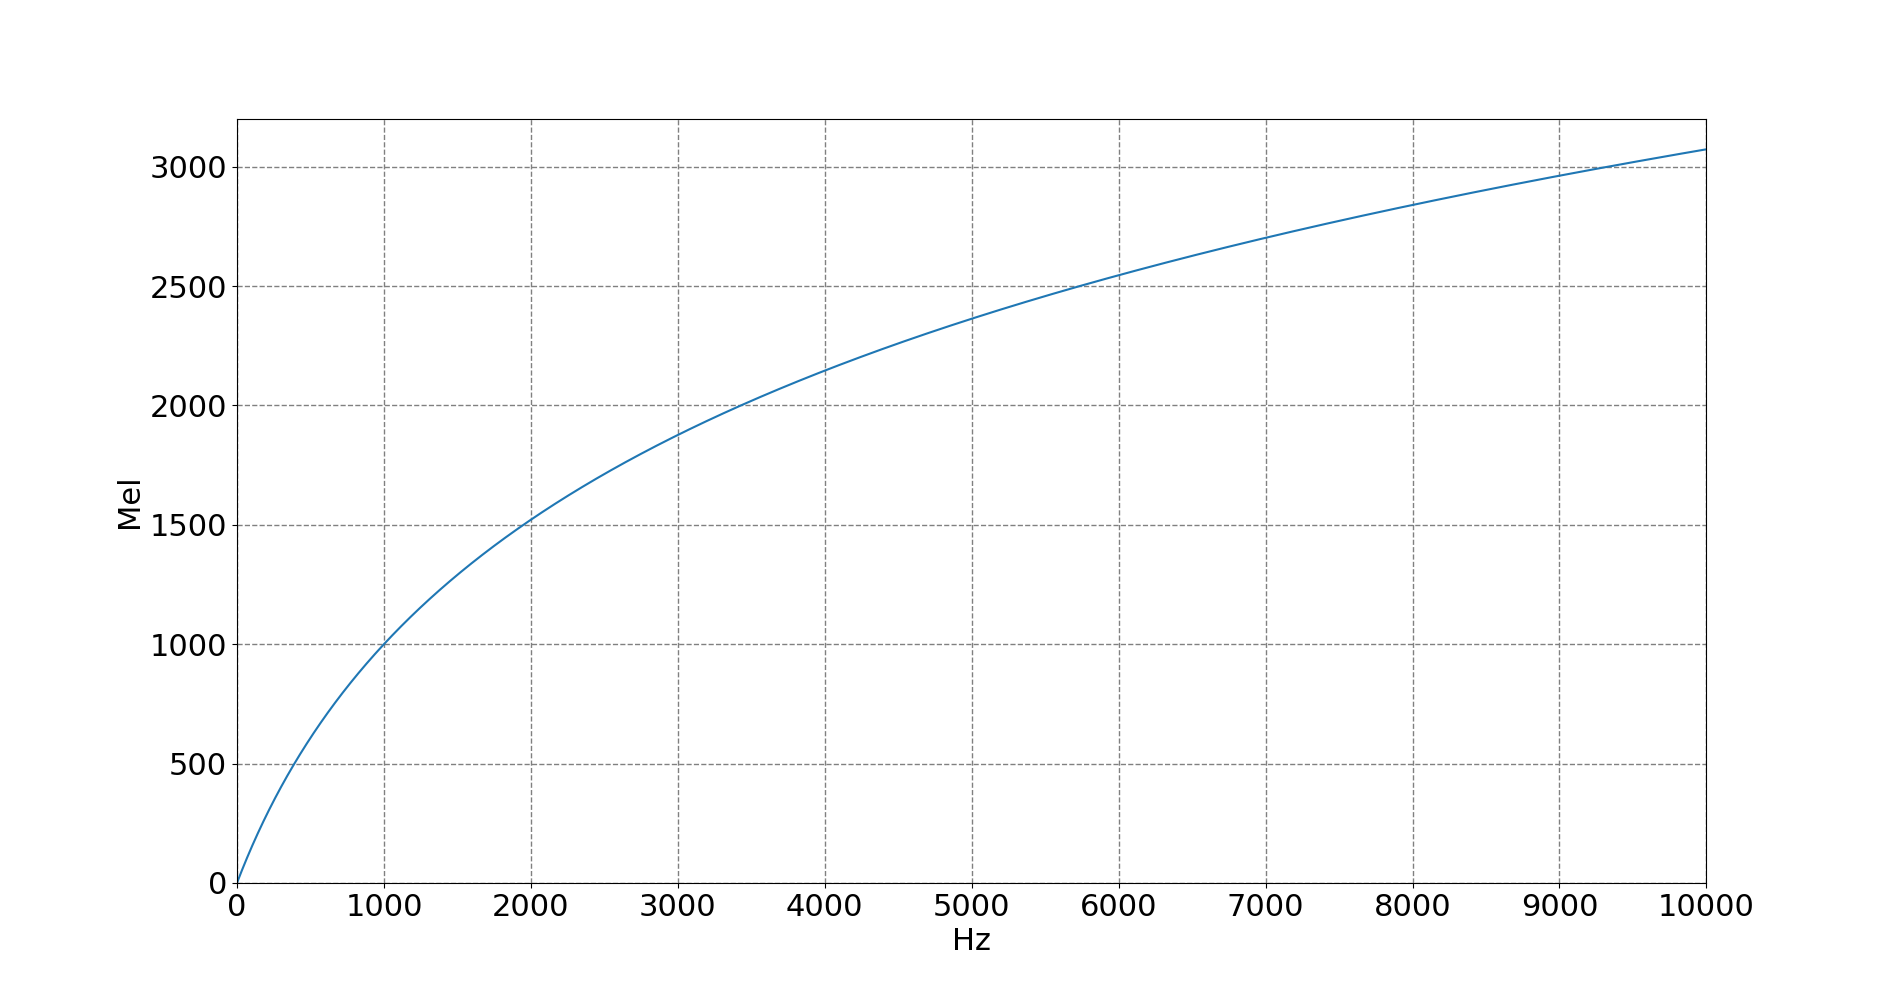
\includegraphics[scale=0.3]{hz_mel.png}\]
	\caption{Сравнение шкал Мел и Гц}
	\label{fig:hz_mel}
\end{figure}


Составляются треугольные Мел-фильтры в виде оконной функции:
\begin{equation}
	H(q,~m)=
	\begin{cases}
		0, 										     & \Phantom \phantom{-}    m < f(q-1)\\
		\dfrac{m-f(q-1)}{f(q)-f(q-1)},   & \Phantom f(q-1) \leq m \leq f(q)\\
		\dfrac{f(q+1)-m}{f(q+1)-f(q)}, & \Phantom f(q) \leq m \leq f(q+1)\\
		0,                                           & \Phantom \phantom{-}   m > f(q+1)\\
	\end{cases}
\end{equation}
для которой $f$ определяется как:
\begin{equation}
	f(a)=\dfrac{N}{w} hz(mel(f_{min})+a \dfrac{mel(f_{max})-mel(f_{min})}{Q+1}),
\end{equation}
где $w$ - частота дискретизации звуковой дорожки, $Q$ - количество коэффициентов MFCC, $f_{min},~f_{max}$ - нижний и верхний пороги частотного диапазона соответственно, $m=\overline{0,N-1}$. Q обычно выбирается в диапазоне 20-40 (26 является своеобразным стандартом).

На рисунке \ref{fig:filters} в качестве примера изображена оконная функция для звуковой дорожки с параметрами $w=44100$ Гц, $f_{min}=0$ Гц, $f_{max}=22050$ Гц, $N=1024$, $Q=13$.

\begin{figure}[H]
	\[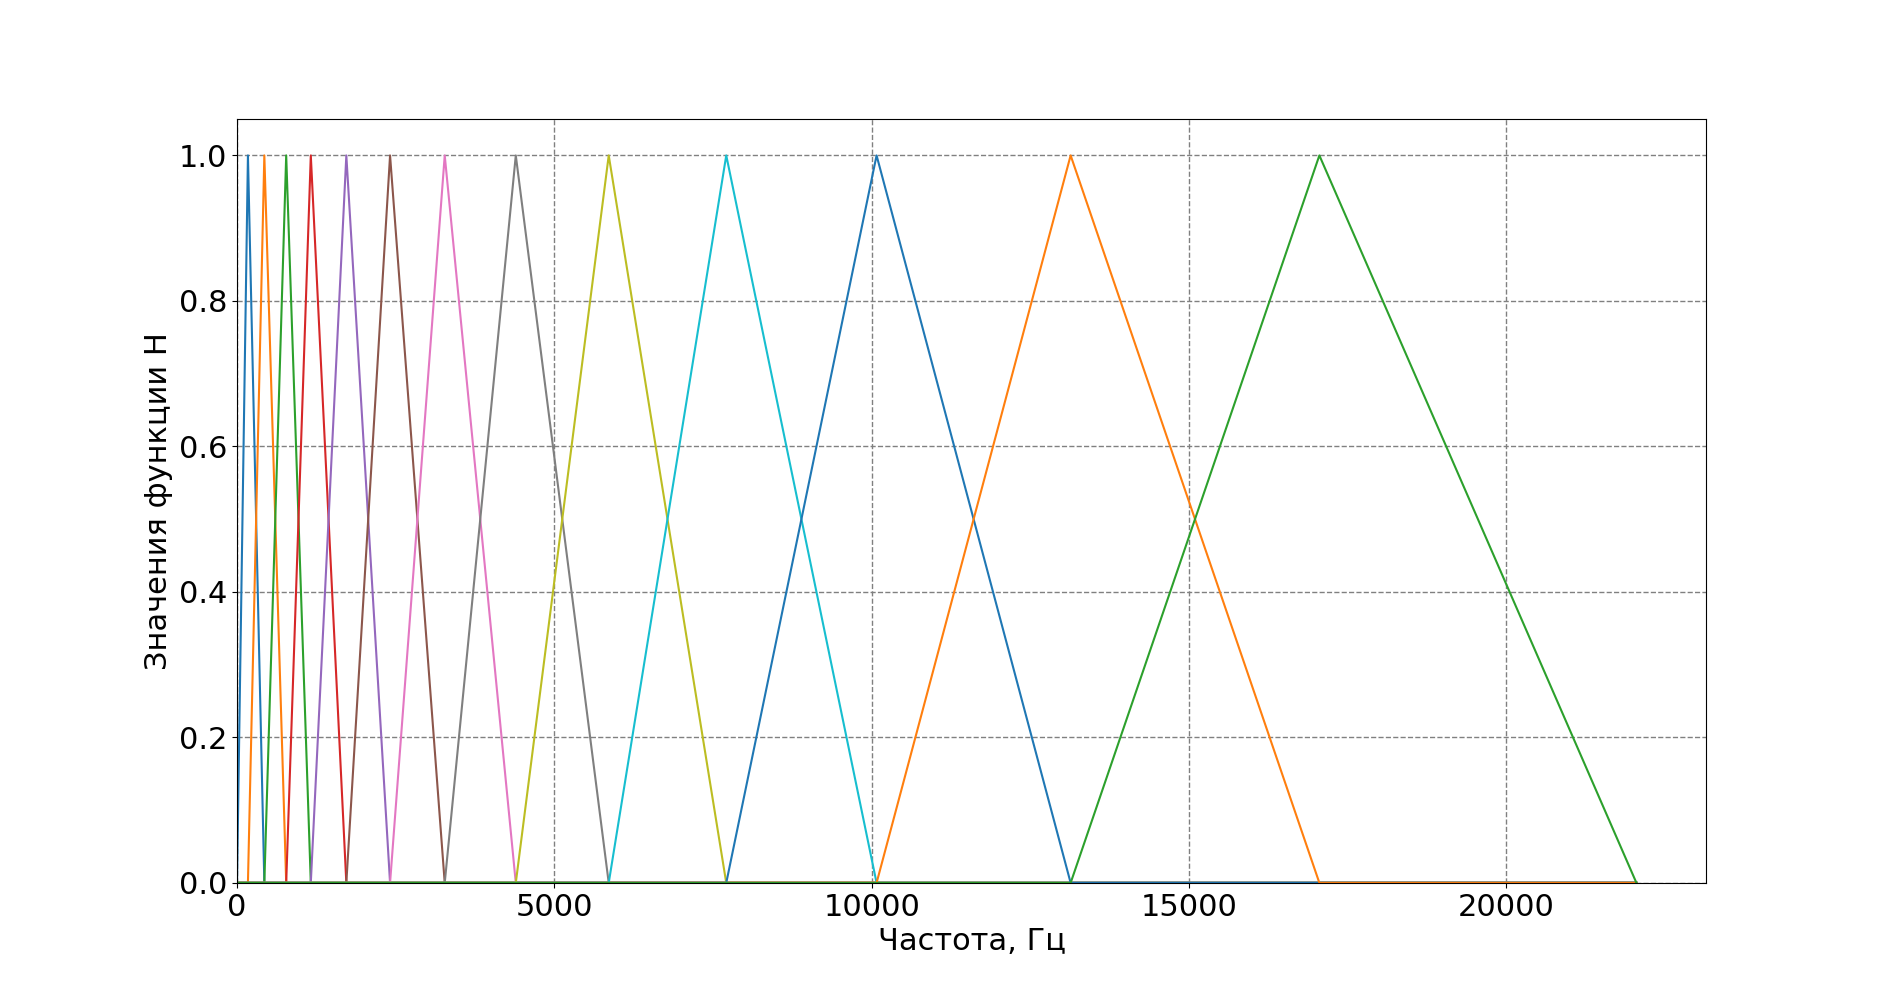
\includegraphics[scale=0.3]{filters.png}\]
	\caption{Оконная функция}
	\label{fig:filters}
\end{figure}

\subsubsection{Получение кепстра сигнала}
Кепстр -  определяется в виде обратного преобразования Фурье от логарифма спектра мощности сигнала:
\begin{equation}
	C_s=\dfrac{1}{2 \pi} \int_{-\inf}^{\inf} ln|(S(w))|^2 \cdot e^{iwq} \,dw,
\end{equation}
где $S(w)$ - спектр входного сигнала.

Кепстр используется в звуковом анализе для оценки основного периода звукового сигнала. В работе \ref{cepstra}
\cite{KeptrumExplanation}

\subsection{Распознавание речевых команд}
\subsubsection{Описание входных и выходных данных модели}
\subsubsection{Архитектура нейронной сети}
\subsubsection{}


\subsection{Распознавание речевых команд}